%!TEX root = ../DSGEnotes.tex
\begin{subappendices}

\section{欧拉公式(复分析)}
\label{sec:euler-complex}

\subsection{欧拉公式和欧拉恒等式}
\label{sec:euler-complex-formula-identityt}

复分析意义上的欧拉公式(Euler formula)\index{Euler formula (complex analysis) \dotfill 欧拉公式}可以表示为
\begin{equation}
  \label{eq:euler-complex-def}
  \exp \left[ i \theta \right] = \cos \theta + i \sin \theta,
\end{equation}
其中$i$是虚数(imaginary number),满足$i = \sqrt{-1}$。欧拉公式的证明,见第\ref{sec:euler-coordinates}节。

欧拉公式的性质,可以从如下引理开始介绍。
\begin{lemma}[$i$的幂是周期方程]
  \label{lemma:i-power-cyclical}
  现在来看$f(x)=i^{x}, \, x=0,1,\ldots$ 的值
  \begin{equation*}
    \begin{pmatrix}
      i^{0}=1, & i^{4}=1, & i^{8}=1, \\
      i^{1}=i, & i^{5}=i, & i^{9}=i, \\
      i^{2}=-1, & i^{6}=-1, & i^{10}=-1, \\
      i^{3}=-i, & i^{7}=-i, & i^{11}=-i, \\
      \vdots & \vdots & \vdots
    \end{pmatrix}
  \end{equation*}
\end{lemma}
不难看出,$i^{x}, \, x=0,1,\ldots$每隔4个数重复一次,因此$f(x)$是一个周期方程。

规律:对于任意整数$x$求$f(x)$,可以将$x$除以$4$,看余数:
\begin{equation*}
  f(x) = i^{n} =
  \begin{cases}
    1 & \text{$\frac{n}{4}$余数是0} \\
    i & \text{$\frac{n}{4}$余数是1} \\
    -1 & \text{$\frac{n}{4}$余数是2} \\
    -i & \text{$\frac{n}{4}$余数是0},
  \end{cases}
\end{equation*}

或者表示为
\begin{equation}
  \label{eq:euler-complex-mod}
  f(x) = i^{x} = i^{x \modd 4}, \, \forall \, x \in \mathcal{Z}.
\end{equation}
其中$\mathcal{Z}_{+}$表示全部正整数集合。$x \modd 4$表示$x$除以4之后的余数。

\begin{lemma}[正弦和余弦的导数]
  \label{lemma:sin-func-derivatives}
现在设$f(x)$是一个正弦函数,满足$f(x)=\sin x$。那么它的$n$次导数,如图\ref{fig:sin-func-derivatives}所示。
\begin{figure}[htbp]
  \caption{正弦函数的导数}
  \centering
  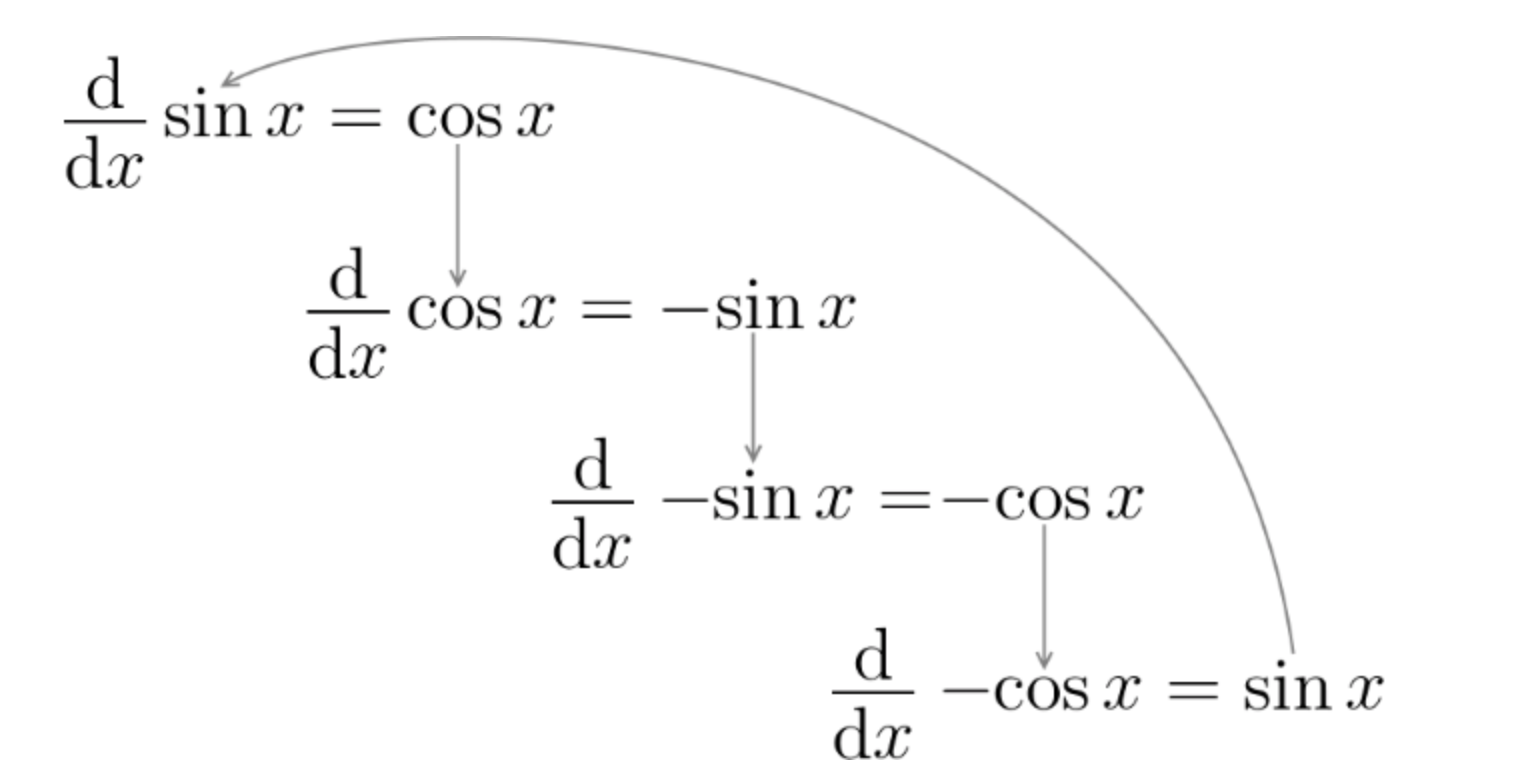
\includegraphics[width=8cm]{./Figures/20180401-sin-cos-derivatives}
  \label{fig:sin-func-derivatives}
%
%  \small{Source: PBOC.}
\end{figure}

\end{lemma}

不难看出,三角函数如正弦的$n$次导数,也是一个以$4$个数为一个周期的周期方程,可以表示为
\begin{equation}
  \label{eq:sin-func-derivatives-mod}
  f^{(n)}(x) = \frac{\mathrm{d}^{n} \sin x}{\mathrm{d} x^{n}}
  = \frac{\mathrm{d}^{n \, \modd \, 4} \sin x}{\mathrm{d} x}
  = \begin{cases}
  \sin x & n \, \modd \, 4 = 0, \\
  \cos x & n \, \modd \, 4 = 1, \\
  - \sin x & n \, \modd \, 4 = 2, \\
  - \cos x & n \,\modd \,4 = 3, \quad \forall \, n \in \mathcal{Z}_{+}.
  \end{cases}
\end{equation}

余弦函数具有类似的性质。此外,对于任意$n \in Z_{+}$,正弦或者余弦函数的$n$阶导数都存在,我们称这种方程为无限可导方程(indefinitely differentiable function)\index{indefinitely differentiable function \dotfill 无限可导方程}。

\begin{lemma}[指数方程的导数]
  \label{lemma:exponential-derivative}
  指数方程的导数是指数方程本身,
  \begin{equation*}
    \frac{\mathrm{d}^{n}}{\mathrm{d} x^{n}} \exp \left[ x \right] = \exp \left[ x \right], \forall \, x, n.
  \end{equation*}
\end{lemma}

\begin{lemma}[泰勒——麦克劳林级数]
  \label{lemma:taylor-maclaurin-series}
  设$f(x)$是一个连续可导方程。对$f(x)$沿着$x=a$做$n$阶的泰勒级数展开,可以得到一个多项式相加的形式,我们称之为泰勒级数(Taylor series)\index{Taylor series \dotfill 泰勒级数}:
  \begin{equation}
    \label{eq:taylor-series-def}
    f \left( x \right) = \frac{f(a)}{0!}
    + \frac{f^{'}(a)}{1!} \left( x - a \right)
    + \frac{f^{''}(a)}{2!} \left( x - a \right)^{2}
    + \ldots
    + \frac{f^{(n)}(a)}{n!} \left( x - a \right)^{n}.
  \end{equation}



%!TEX root = ../DSGEnotes.tex
\begin{figure}[htbp]
  \centering  %居中
  \subfigure[$n=1$]{  %第一张子图
  \begin{minipage}{7cm}
    \centering  %子图居中
    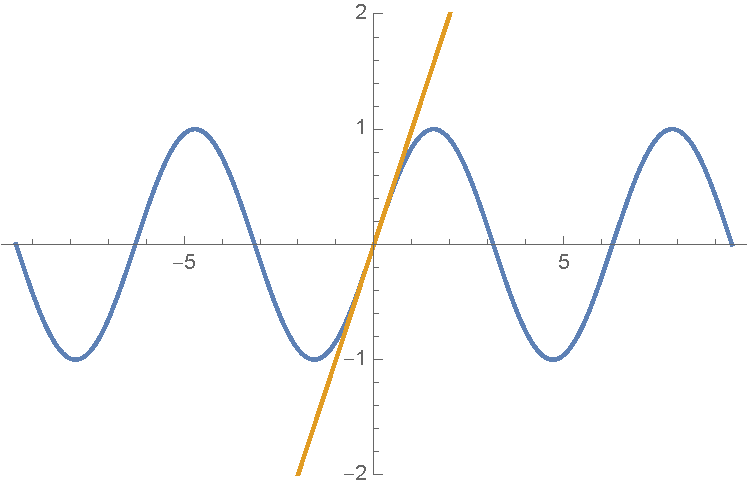
\includegraphics[scale=0.5]{./Figures/20180315-taylor-n1} %以pic.jpg的0.5倍大小输出
  \end{minipage}}
  \subfigure[$n=3$]{  %第二张子图
  \begin{minipage}{7cm}
    \centering  %子图居中
    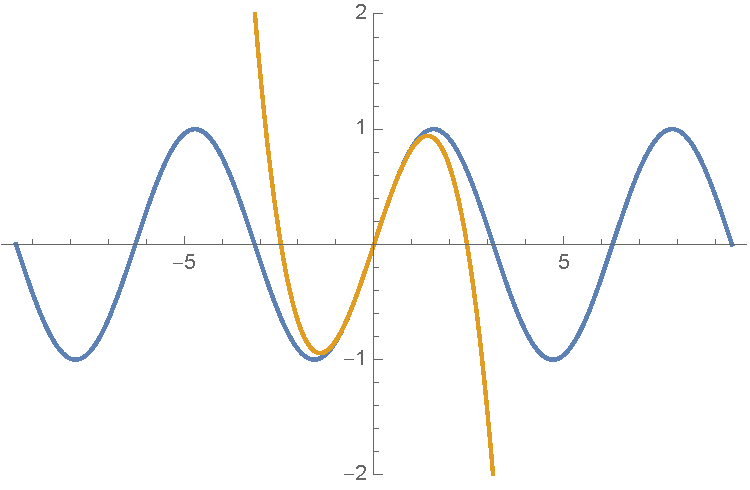
\includegraphics[scale=0.5]{./Figures/20180315-taylor-n3} %以pic.jpg的0.5倍大小输出
  \end{minipage}}
  \subfigure[$n=5$]{  %第二张子图
  \begin{minipage}{7cm}
    \centering  %子图居中
    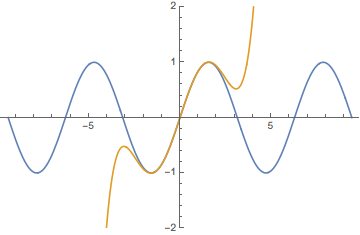
\includegraphics[scale=0.5]{./Figures/20180315-taylor-n5} %以pic.jpg的0.5倍大小输出
  \end{minipage}}
  \subfigure[$n=7$]{  %第二张子图
  \begin{minipage}{7cm}
    \centering  %子图居中
    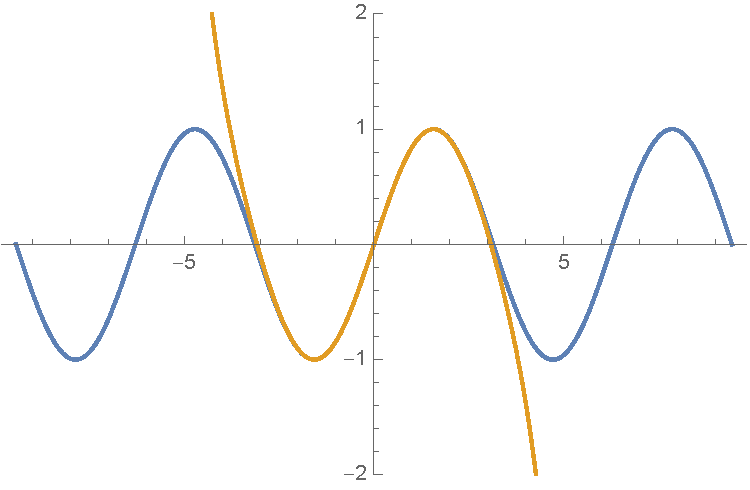
\includegraphics[scale=0.5]{./Figures/20180315-taylor-n7} %以pic.jpg的0.5倍大小输出
  \end{minipage}}
  \subfigure[$n=9$]{  %第二张子图
  \begin{minipage}{7cm}
    \centering  %子图居中
    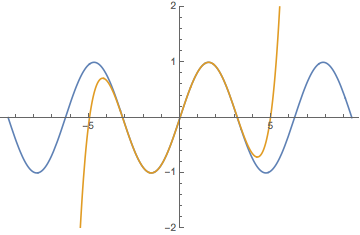
\includegraphics[scale=0.5]{./Figures/20180315-taylor-n9} %以pic.jpg的0.5倍大小输出
  \end{minipage}}
  \subfigure[$n=11$]{  %第二张子图
  \begin{minipage}{7cm}
    \centering  %子图居中
    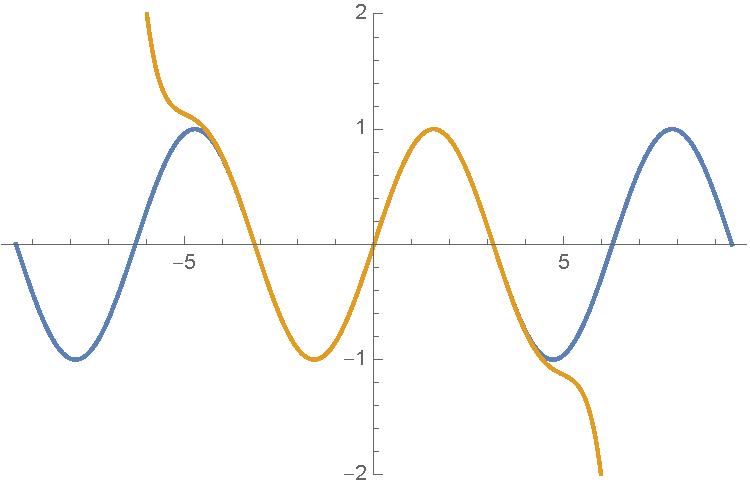
\includegraphics[scale=0.5]{./Figures/20180315-taylor-n11} %以pic.jpg的0.5倍大小输出
  \end{minipage}}
  \subfigure[$n=13$]{  %第二张子图
  \begin{minipage}{7cm}
    \centering  %子图居中
    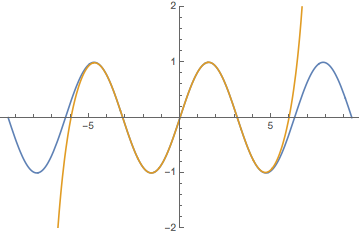
\includegraphics[scale=0.5]{./Figures/20180315-taylor-n13} %以pic.jpg的0.5倍大小输出
  \end{minipage}}
  \subfigure[$n=15$]{  %第二张子图
  \begin{minipage}{7cm}
    \centering  %子图居中
    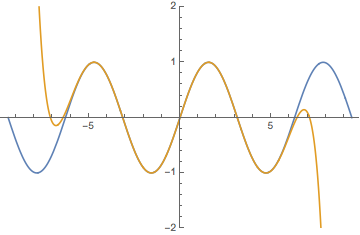
\includegraphics[scale=0.5]{./Figures/20180315-taylor-n15} %以pic.jpg的0.5倍大小输出
  \end{minipage}}
  \caption{麦克劳林级数的示例:对$\sin(x)$(蓝色曲线)沿着$x_{0}=0$作$n$阶泰勒级数展开(红色曲线)。} %大图名称
  \label{fig:maclaurin-series-example} %图片引用标记\end{figure}
%  \end{minipage}
\end{figure}

不难看出,$n$的值越大,近似的精度越高,如图\eqref{fig:maclaurin-series-example}所示。当$n \rightarrow \infty$时,近似是完全精确的。

当$a=0$时,泰勒级数变为沿着$x=a=0$的点作$n$阶泰勒展开,所生成的级数称麦克劳林级数(Maclaurin series)\index{Taylor-Maclaurin series \dotfill 麦克劳林级数}:
\begin{equation}
  \label{eq:taylor-maclaurin-series-def}
  f \left( x \right) = \frac{f(0)}{0!}
  + \frac{f^{'}(0)}{1!} \left( x  \right)
  + \frac{f^{''}(0)}{2!} \left( x \right)^{2}
  + \ldots
  + \frac{f^{(n)}(0)}{n!} \left( x \right)^{n}.
\end{equation}
\end{lemma}

\begin{lemma}[指数方程的麦克劳林级数(幂级数)]
  \label{lemma:exponential-maclaurin}
  现在设$f(x)= \exp x$。对应的麦克劳林级数展开由\eqref{eq:taylor-maclaurin-series-def}变为
\begin{equation}
  \label{eq:exponential-maclaurin-series-def}
  \begin{split}
    f \left( x \right) = \exp x & = \frac{f(0)}{0!}
    + \frac{f^{'}(0)}{1!} \left( x  \right)
    + \frac{f^{''}(0)}{2!} \left( x \right)^{2}
    + \ldots
    + \frac{f^{(n)}(0)}{n!} \left( x \right)^{n} \\
    & = 1 + \frac{x}{1!} + \frac{x^{2}}{2!} + \frac{x^{3}}{3!} + \frac{x^{4}}{4!} + \ldots \\
    & = \sum_{n=0}^{\infty} \frac{x^{n}}{n!}.
  \end{split}
\end{equation}
又称幂级数(power series)\index{power series \dotfill 幂级数}。
\end{lemma}

\begin{lemma}[正弦的麦克劳林级数]
  \label{lemma:sin-maclaurin-series}
  现在设$f(x) = \sin x$,对应的麦克劳林级数展开由\eqref{eq:taylor-maclaurin-series-def}变为
  \begin{equation}
    \label{eq:sin-cos-maclaurin-series}
    \begin{split}
      f \left( x \right) = \sin x & = \frac{f(0)}{0!}
      + \frac{f^{'}(0)}{1!} \left( x  \right)
      + \frac{f^{''}(0)}{2!} \left( x \right)^{2}
      + \ldots
      + \frac{f^{(n)}(0)}{n!} \left( x \right)^{n} \\
      & = \sin 0 + \frac{\cos 0}{1!} x
      + \frac{- \sin 0}{2!} x^{2}
      + \frac{- \cos 0}{3!} x^{3} + \ldots \\
      & = x - \frac{x^{3}}{3!} + \frac{x^{5}}{5!} - \frac{x^{7}}{7!} + \frac{x^{9}}{9!} - \ldots \\
      & = \sum_{n=0}^{\infty} \left( -1 \right)^{n} \frac{x^{2n+1}}{ \left( 2n + 1 \right)!}.
    \end{split}
  \end{equation}
\end{lemma}

\begin{lemma}[余弦的麦克劳林级数]
  \label{lemma:cos-maclaurin-series}
  类似地,若设$f(x)=\cos(x)$,有余弦的麦克劳林级数
  \begin{equation}
    \label{eq:cos-maclaurin-series}
  f(x) =   \cos x = 1 - \frac{x^{2}}{2!} + \frac{x^{4}}{4!} - \frac{x^{6}}{6!} + \frac{x^{8}}{8!} - \ldots = \sum_{n=0}^{\infty} \left( -1 \right)^{n} \frac{x^{2n}}{\left( 2n \right)!}.
  \end{equation}
\end{lemma}

\begin{lemma}[欧拉恒等式]
  \label{sec:euler-complex-identity}
  根据指数方程的麦克劳林级数(幂级数)引理(Lemma \ref{lemma:exponential-maclaurin}),将式\eqref{eq:exponential-maclaurin-series-def}中全部$x$都替换为$i x$,则有
  \begin{equation}
    \label{eq:euler-complex-identity}
    \begin{split}
      \exp \left[ i x \right] = \sum_{n=0}^{\infty} \frac{\left( i x \right)^{n}}{n!}
      & = 1 + \frac{\left( i \right) x}{1!}
      + \frac{\left( -1 \right) x^{2}}{2!}
      + \frac{\left( -i \right) x^{3}}{3!}
      + \frac{ x^{4}}{4!}
      + \ldots \\
      & = 1 + i \frac{x}{1!} - \frac{x^{2}}{2!}
      - i  \frac{x^{3}}{3!}
      + \frac{x^{4}}{4!}
      + i \frac{x^{5}}{5!}
      - \frac{x^{6}}{6!}
      - i \frac{x^{7}}{7!}
      + \ldots \\
      & =
      \left(
      1 - \frac{x^{2}}{2!} + \frac{x^{4}}{4!} - \frac{x^{6}}{6!} + \ldots
      \right)
      + i \left(
      x - \frac{x^{3}}{3!} + \frac{x^{5}}{5!} - \frac{x^{7}}{7!} + \ldots
      \right) \\
      & = \cos x + i \sin x.
    \end{split}
  \end{equation}
  又称欧拉恒等式(Euler identity)\index{Euler identity \dotfill 欧拉恒等式}。
\end{lemma}

\subsection{欧拉公式的作用}
\label{sec:euler-complex-uses}

欧拉公式、欧拉恒等式有什么用途?

\subsubsection{复数的坐标形式}
\label{sec:euler-coordinates}
一个复数(complex number)可以表示为一个时部和一个虚部相加的形式,例如对于复数$z$我们有
\begin{equation*}
\begin{split}
    z & = \Re(z) + i \Im(z) = x + i y, \quad x,y \in \mathbb{R}, \, i = \sqrt{-1}.
\end{split}
\end{equation*}

以实部为横轴,以虚部为纵轴,可以将$z$表示为复平面(complex plane)中的$(x,y)$点。我们常用模(magnitude)和角(angle),对应$\left\{ r, \theta \right\}$,来在复平面中表示$z$,如图\eqref{fig:euler-complex-plane}所示。

\begin{figure}[htbp]
  \caption{正弦函数的导数}
  \centering
  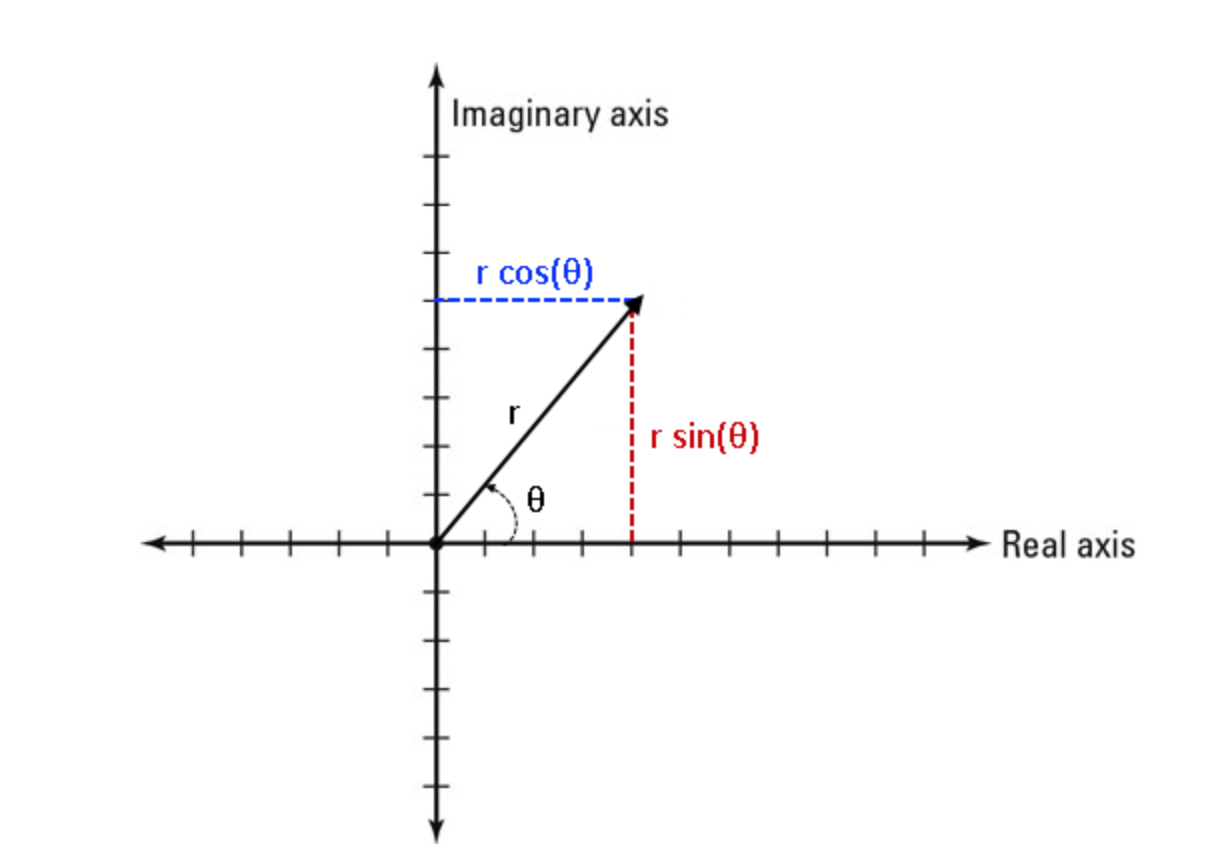
\includegraphics[width=8cm]{./Figures/20180401-complex-plane}
  \label{fig:euler-complex-plane}
%
%  \small{Source: PBOC.}
\end{figure}

由三角函数关系可得$x = r \cos \theta, \, y = r \sin \theta$,那么结合欧拉恒等式(Lemma \ref{sec:euler-complex-identity})可得
\begin{equation}
  \label{eq:euler-coordinates-complex-plane-z}
\begin{split}
    & z = x + i y = r \cos \theta + i r \sin \theta = r \left( \cos \theta + i \sin \theta \right) = r \exp \left( i \theta \right), \\
    & \hookrightarrow x + i y = r \exp \left( i \theta \right), \quad x = r \cos \theta, \, y = r \sin \theta,
\end{split}
\end{equation}
就是欧拉公式,将一个复数$z$写为关于夹角$\theta$和模$r$的三角方程

\subsubsection{复数的乘除}
\label{sec:euler-complex-multi-divid}
复数的乘除法如
\begin{equation*}
\begin{split}
  \left( a + b i \right) \left( c + d i \right)
  & = ac + a d i + b c i - b d = \left( ac - bd \right) + \left( ad + bc \right) i.
\end{split}
\end{equation*}

另一种算法时,假定要将两个指数方程相乘,满足
\begin{equation*}
  a \exp \left( i \theta \right) \cdot b \exp \left( i \theta \phi \right) = ab \exp \left[ i \left(\theta + \phi \right) \right],
\end{equation*}
即是说,两个复数相乘,就是分别将二者的模和夹角相乘。上式可以进一步写为
\begin{equation*}
  a \exp \left( i \theta \right) \cdot b \exp \left( i \theta \phi \right) = ab \left[ \cos \left( \theta + \phi \right) + i \sin \left( \theta + \phi \right) \right].
\end{equation*}

除法的操作类似。

\subsubsection{对复数的取幂}
\label{sec:euler-complex-exponentiation}

假设我们要计算$\left( a+bi \right)^{n}$的值。常见的简化方法之一是借助复数的形式
\begin{equation}
  \label{eq:euler-complex-exponentiation}
  \begin{split}
    \left( a+bi \right)^{n} & = \left[ r \exp
    \left(
    i \theta
    \right)
    \right]^{n}
    = r^{n} \exp \left( i \theta n \right)
    = r^{n} \left[ \cos \left( \theta n \right) + i \sin \left( \theta n \right) \right], \quad \forall \, n \in \mathbb{Z}_{+},
  \end{split}
\end{equation}
将一个复数的求幂运算(exponentiation)\index{exponentiation (complex analysis) \dotfill 取幂(复分析)}转换为幂指数的形式,又称棣莫弗定理(De Moivre Theorem)\index{De Moivre Theorem \dotfill 棣莫弗定理}。

前面介绍了如何将一个复数表示为幂指数形式,现在来看如何将一个实数表示为一个复数。已知欧拉公式\eqref{eq:euler-complex-def}
\begin{equation*}
  \exp \left[ i x \right] = \cos x + i \sin x,
\end{equation*}
将其中的$x$替换为$x \ln b$
\begin{equation*}
  \exp \left( i x \ln b \right) = \cos \left( x \ln b \right) + i \sin \left( x \ln b \right) = b^{i x},
\end{equation*}
那么,若对某个复数$y+ix$作幂,求$b^{y+ix}$的值,可计算如下
\begin{equation}
  \label{eq:euler-complex-exponentiation-xyi}
  b^{y+ix} = b^{y} \, b^{ix} = b^{y}
  \left[
  \cos \left( x \ln b \right) + i \sin \left( x \ln b \right)
  \right].
\end{equation}

举例:
\begin{equation*}
  5^{3+2i} = 5^{3} \, 5^{2i} = 5^{3} \left[ \cos \left( 2 \ln 5 \right) + i \sin \left( 2 \ln 5 \right) \right] \approx - 124.63 - 9.65 i.
\end{equation*}

\subsubsection{复值夹角}
\label{sec:euler-complex-angle-conjugate}
根据欧拉公式,可以进一步引出复值夹角(complex angle)\index{complex angle \dotfill 复值夹角}和三角方程的概念。先来看复值夹角。具体说来,前面我们所涉及到的正弦、余弦方程如$\sin(x)$,是对实数$x$的计算。如果要对一个复数求正弦余弦,该怎么操作?

对欧拉恒等式\eqref{eq:euler-complex-identity}作调整,用$-x$替代$x$,有
\begin{equation}
  \label{eq:euler-complex-identity-conjugate}
\begin{split}
  & \exp \left( i x \right) = \cos x + i \sin \left( x \right), \text{原方程}\\
  & \exp \left( - i x \right) = \cos x - i \sin \left( x \right) \text{复共轭},
\end{split}
\end{equation}
将一个复数的虚部变更符号(例如由正变为负),所组成的新的复数,称为原复数的复共轭(complex conjugate)\index{complex conjugate \dotfill 复共轭}。

现在对欧拉恒等式\eqref{eq:euler-complex-identity}及其复共轭\eqref{eq:euler-complex-identity-conjugate}相加和相减,得
\begin{align}
  \label{eq:euler-complex-identity-conjugate-plus}
  & \exp \left( i x \right) - \exp \left( - i x \right) = 2 i \sin x,  \Longleftrightarrow \sin x = \frac{\exp \left( i x \right) - \exp \left( - i x \right)}{2 i}, \\
  \label{eq:euler-complex-identity-conjugate-minus}
  & \exp \left( i x \right) + \exp \left( - i x \right) = 2 \cos x, \Longleftrightarrow \cos x = \frac{\exp \left( i x \right) + \exp \left( - i x \right)}{2},
\end{align}
即,我们得到了一组用指数(和虚数)表示的正弦、余弦方程。

调整\eqref{eq:euler-complex-identity-conjugate-plus}-  \eqref{eq:euler-complex-identity-conjugate-minus},用$ix$替换原式中的$x$,并且分子分母同时乘以$i$得
\begin{align}
  \label{eq:euler-complex-identity-conjugate-plus-i}
  & \sin \left( ix \right) = \frac{\exp \left( i^{2} x \right) - \exp \left( - i^{2} x \right)}{2 i^{2}} \frac{i}{i}
  = \frac{
  i \left[ \exp \left( x \right) - \exp \left( - x \right) \right]
  }{2} \equiv i \sinh x, \\
  \label{eq:euler-complex-identity-conjugate-minus-i}
  & \cos \left( ix \right) = \frac{\exp \left( i^{2} x \right) + \exp \left( - i^{2} x \right)}{2} \frac{i}{i} = \frac{
  \left[ \exp \left( x \right) + \exp \left( - x \right) \right]
  }{
  2
  } \equiv \cosh x,
\end{align}
其中$\sinh(x), \cosh(x)$分别称双曲线正弦方程和双曲线余弦方程(hyperbolic sine/cosine function)\index{hyperbolic function!sine \dotfill 双曲线正弦方程}\index{hyperbolic function!cosine \dotfill 双曲线余弦方程},如图  \ref{fig:sinh-cosh-function}。值得注意的是右图:任何虚数的余弦都是一个实数,原本的虚部消失不见。

\begin{figure}[htbp]
  \caption{双曲正弦/余弦方程,$x \in \left[ -3 \pi, 3 \pi\right]$}
  \centering
  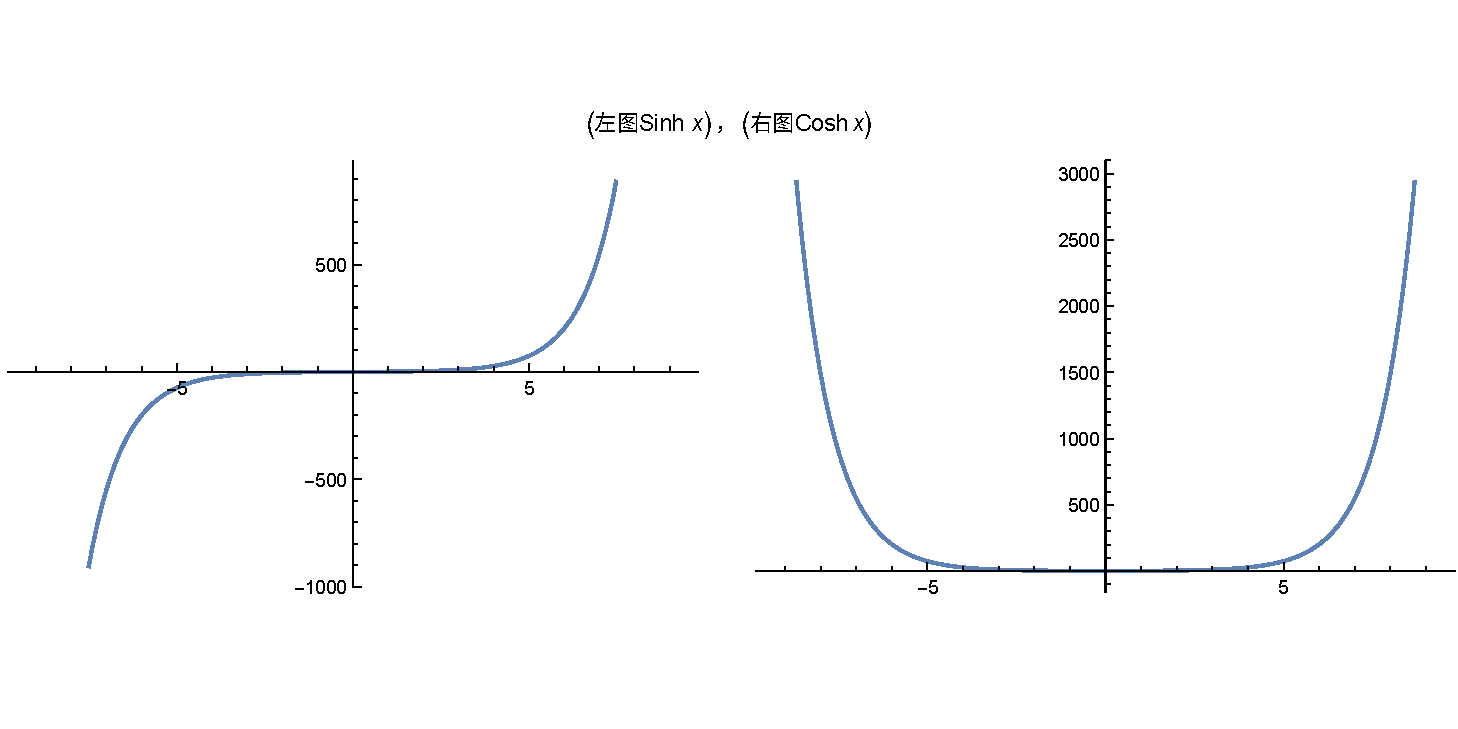
\includegraphics[width=12cm]{./Figures/20180401-sinh-cosh-x}
  \label{fig:sinh-cosh-function}
%
%  \small{Source: PBOC.}
\end{figure}

在此基础上,我们可以回答本节初提出的问题,如何计算一个复数的正弦/余弦,如$\sin \left( a + bi \right)$。
已知$\sin(a+b) = \sin a \cos b + \cos a \sin b$,并且$\sinh x, \cosh x$的定义如\eqref{eq:euler-complex-identity-conjugate-plus-i}-\eqref{eq:euler-complex-identity-conjugate-minus-i}所示。那么,用$bi$替换原式中的$b$,可得复数的正弦计算式
\begin{equation}
  \label{eq:complex-sin-abi}
\begin{split}
  \sin \left( a + b i \right) & = \sin a \cos \left( i b \right) + \cos a  \sin \left( i b \right) \\
  & = \sin a \cosh b + i \cos a \sinh b.
\end{split}
\end{equation}

余弦:$\cos \left( a + b \right) = \cos a \cos b - \sin a \sin b$。用$bi$替换$b$
\begin{equation}
  \label{eq:complex-cos-abi}
\begin{split}
  \cos \left( a + bi \right) & = \cos a \cos \left( ib\right) - \sin a \sin \left( i b \right) \\
  & = \cos a \cosh b - i \sin a \sinh b.
\end{split}
\end{equation}

举例:
\begin{equation*}
  \cos \left( 3 + 4 i \right)
  = \cos (3) \cosh (4) - i \sin (3) \sinh (4)
  \approx -27.03 + 3.85 i.
\end{equation*}
%\subsubsection{三角方程}
%三角方程(Trigonometry)

\section{高斯核方程}
\label{sec:kernel-analysis}

\subsection{高斯核}
\label{sec:kernel-gaussian}
%mchung teaching notes.
一个常见的高斯核方程(kernel function!Gaussian)\index{kernel function!Gaussian \dotfill 高斯核方程},随着维度的不同,可以表示如下
\begin{align}
  \label{eq:kernel-gaussian-dim1}
  G^{(1)} \left( x ; \sigma \right) & = \frac{1}{\sqrt{2 \pi} \sigma}
  \exp \left( - \frac{x^{2}}{2 \sigma^{2}} \right), \\
  \label{eq:kernel-gaussian-dim2}
  G^{(2)} \left( x,y; \sigma \right)
  & = \frac{1}{2 \pi \sigma^{2}}
  \exp \left(  - \frac{x^{2} + y^{2}}{2 \sigma^{2}} \right), \\
  \vdots & \nonumber \\
  \label{eq:kernel-gaussian-dimN}
  G^{(N)} \left( \vec{x} ; \sigma \right)
  & = \frac{1}{\left(\sqrt{2 \pi} \sigma \right)^{N}}
  \exp \left(
  - \frac{
  \left| \vec{x} \right|^{2}
  }{
  2 \sigma^{2}
  }
  \right),
\end{align}
其中
\begin{itemize}
\item $\sigma > 0$表示高斯核的带宽(bandwidth),统计学中也将上式称为高斯概率密度方程(Gaussian probability density function)\index{probability density function (PDF)!Gaussian\dotfill 高斯概率密度方程}——对应地,称$\sigma$为标准差,$\sigma^{2}$为方差。
\item $\left\{ x \right\}$,$\left\{ x,y \right\}$分别表示1维和2维空间参数。$N$维空间参数往往用向量$\vec{x}$进行简化表示。
\item 空间参数和带宽参数之间的分号是常见的表达方式,提醒人们两者的含义不同。指数项中乘以$1/2$也是为了表述方便。
\end{itemize}

\subsection{标准化}
\label{sec:kernel-gaussian-normalization}
以1维高斯核方程\eqref{eq:kernel-gaussian-dim1}为例,前面的常数项$\frac{1}{\sqrt{2 \pi} \sigma}$是标准化常数,引入这个常数项是由于对$\exp \left( - \frac{x^{2}}{2 \sigma^{2}} \right)$沿着$x \in \left( - \infty, \infty \right)$求积,其值不等于$1$
\begin{equation*}
  \int_{-\infty}^{\infty} \exp \left( -
  \frac{x^{2}}{2 \sigma^{2}}
  \right) \mathrm{d} x = \sqrt{2 \pi} \sigma \neq 1.
\end{equation*}

在作标准化处理后,高斯核成为一个标准化的核方程,即满足
\begin{equation*}
  \int_{-\infty}^{\infty} G^{(1)} \left( x; \sigma \right)
  \, \mathrm{d} x = 1, \forall \, \sigma,
\end{equation*}
另一方面,增加带宽$\sigma$的值会显著降低$G^{(1)} \left( x ; \sigma \right)$的振幅(amplitude),例如$\sigma$取$0.3,1,2$三组不同的值,对应高斯方程\eqref{eq:kernel-gaussian-dim1}在$[-1.5\pi, 1.5\pi]$的形状,见图\ref{fig:gaussian-amplitude-sigma},图中取下下方阴影部分的面积均为$1$。
\begin{figure}[htbp]
  \caption{高斯核方程的振幅随带宽的增加而显著降低}
  \centering
  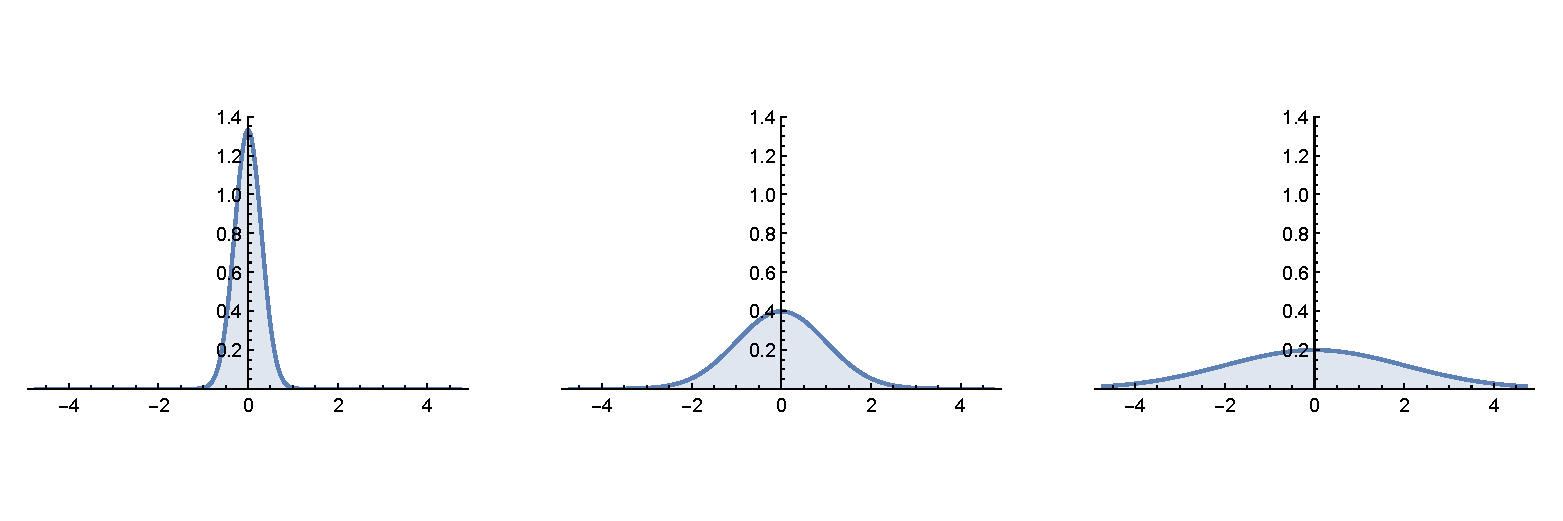
\includegraphics[width=12cm]{./Figures/20180404-gaussian-amplitude-sigma}
  \label{fig:gaussian-amplitude-sigma}
%
%  \small{Source: PBOC.}
\end{figure}

\subsection{瀑布特征}
\label{sec:kernel-gaussian-cascade}
将两个高斯核作卷积(convolution),可以得到一个新的高斯核方程,新方程具有与原方程相似的特性:
\begin{equation}
  \label{eq:kernel-gaussian-convolution}
  G_{1}\left( \vec{x_{1}}; \sigma_{1} \right)
  \, G_{2}\left( \vec{x_{2}}; \sigma_{2} \right)
  =  G_{new} \left( \vec{x} ; \sqrt{\sigma_{1}^{2} + \sigma_{2}^{2}} \right),
\end{equation}
我们称这种特性为自相似性(self-similarity)\index{self-similarity \dotfill 自相似性},高斯核方程就是这样一种自相似方程。

高斯方程的卷积是线性运算,那么高斯方程卷积的卷积也是线性运算,以此类推,这称为瀑布特性(cascade property)。

\subsection{带宽参数}
\label{sec:kernel-gaussian-bandwidth}
由于$\sigma_{1}^{2}+\sigma_{2}^{2}$较难直接计算,我们常常用$t \equiv 2 \sigma^{2}$的方式来做近似参数化处理。对于$N$维高斯核方程而言,有
\begin{equation*}
  G^{(N)} \left( \vec{x}; t\right) = \frac{1}{\left( \pi t \right)^{\frac{N}{2}}} \exp \left( - \frac{x^{2}}{t} \right).
\end{equation*}

如果$N=3$即向量$\vec{x}$中包括三组数据$\left\{x_{1},x_{2},x_{3}\right\}$,那么
\begin{equation*}
  \frac{\partial \mathcal{L}}{\partial t} = \sum_{i=1}^{3} \frac{\partial^{2} L}{\partial x_{i}^{2}},
\end{equation*}
即方差。


为了更好了解高斯核方程的自相似特征,我们引入一个无量纲(dimensionless)参数空间$\tilde{x} = \frac{x}{ \sqrt{2} \sigma}$来对$x$轴做"参数化"处理,对应的高斯核方程为
\begin{equation*}
\begin{split}
    G^{(N)} \left( \tilde{x}; \sigma \right) & = \frac{1}{\left( \sigma \sqrt{2 \pi} \right)^{N}} \exp \left( - \tilde{x}^{2} \right), \\
    G^{(N)} \left( \tilde{x}; t \right) & =
    \frac{1}{\left(\pi t\right)^{\frac{N}{2}}} \exp \left( - \tilde{x}^{2} \right),
\end{split}
\end{equation*}
两式等价。换句话说,沿着空间轴($x$轴)以$\sigma$的倍数为步长单位行走,其中所有的核方程都有相同的大小,又称带宽。

需要注意的是,带宽相同的高斯核,其振幅未必相同——这是由标准化计算流程所决定的。

在新的空间坐标系$\tilde{x}$中漫步,每一步的步长等于$\sqrt{2} \sigma$。对应地,我们称之为自然高斯核方程(natural) $G^{(N)} \left( \tilde{x} ; \sigma \right)$,对应的新坐标$\tilde{x} = \frac{x}{\sqrt{2} \sigma}$称为自然坐标。通过这种处理方法,可以从空间坐标系中去除方差$\sigma$,从而使得高斯核方程$G^{(N)}$彼此相似,区别只在于其(卷积$\tilde{x}$中的内方差)。

高斯核方程的值域是$\left( - \infty, \infty \right)$,但在现实应用中, $\left| x \right| > \sigma$的高斯核往往小到可以忽略不计。(如Mathematica计算$\sigma = 1, \, x = 5 \sigma$的高斯核)。

\subsection{一些方程}
\label{sec:kernel-gaussian-prep}
高斯核方程是一个半局部(semi-local)方程。之所以不是全局部的方程,是由于其卷积内部仍然存在着方差$\sigma$,从而使得空间里存在一个高斯加权范围(Gaussian weighted extend)。在下一节我们将提出一个通用方程来将其全局化,在此之前,本节先介绍一些基础知识。

当将方差$\sigma$取其极限值$\lim \sigma \rightarrow 0$时,高斯核方程变成Delta方程的一种特殊形式,又称德尔塔-狄拉克方程(Delta-Dirac function)\index{Delta Dirac function \dotfill 狄拉克方程} $\delta(\cdot)$:
\begin{equation}
  \label{eq:kernel-gaussian-dirac-def}
\begin{split}
  \delta \left( \tilde{x} \right) \coloneqq \lim_{\sigma \rightarrow 0} G(\tilde{x}; \sigma) & = \lim_{\sigma \rightarrow 0} \frac{1}{\sqrt{2 \pi} \sigma}
  \exp \left( - \tilde{x}^{2} \right), \quad \tilde{x} = \frac{x}{\sqrt{2} \sigma} \\
  & = \lim_{\sigma \rightarrow 0} \frac{1}{\sqrt{2 \pi} \sigma} \exp \left( - \frac{x^{2}}{2 \sigma^{2}} \right) \\
  & = \begin{cases}
  \infty & x =0, \\
  0 & x \neq 0.
  \end{cases}
\end{split}
\end{equation}

在数学上,狄拉克方程$\delta \left( \cdot \right)$常称为取样方程。例如,对$f(x)$取$x=a$时的值,$a$是个常数。设$f(x)$在$x=a$处连续,可表示为如下求积形式
\begin{equation*}
  \int_{-\infty}^{\infty} \delta \left( x - a \right) \, f(x) \, \mathrm{d} x = f \left( a \right).
\end{equation*}

狄拉克方程的导数可定义如下
\begin{equation}
  \label{eq:kernel-gaussian-dirac-derivatives}
  \begin{split}
    \int_{-\infty}^{\infty} \delta^{'} (x) f(x) \, \mathrm{d} x & = - f^{'}(0),
    \\
    \int_{-\infty}^{\infty} \delta^{''} (x) f(x) \, \mathrm{d} x & = - f^{''}(0).
  \end{split}
\end{equation}

将全部$\left( -\infty, x \right]$区间中的高斯核加总,称为累积高斯方程(culmulative Gaussian kernel function)\index{kernel function!Gaussian, culmulative \dotfill 累积高斯核方程},又称误差方程(error function)\index{error function \dotfill 误差方程}
\begin{equation}
  \label{eq:kernel-gaussian-culmulative}
  err \left( x; \sigma \right) \coloneqq \int_{0}^{x} \frac{1}{\sqrt{2 \pi} \sigma} \exp \left( - \frac{y^{2}}{2 \sigma^{2}}\right) \, \mathrm{d} y,
\end{equation}
在Mathematica中运行程序,返回值$\frac{1}{2} Erf\left[ \frac{x}{\sqrt{2 \pi} \sigma} \right]$。$Erf[]$是Mathematica内建的高斯误差计算方程,前面乘以1/2是因为求积区间只是$[0,x]$,是$[-x,x]$的一半。

现在逐渐减少$\sigma$的值,$1.0 \rightarrow 0.1$。不难看出,随着$\sigma$越来越接近于$0$,在$x=0$附近就越会出现较大的跃动,如图\eqref{fig:gaussian-kernel-sigma-value}。
\begin{figure}[htbp]
  \caption{误差方程(累积高斯方程)随$\sigma$值的变化}
  \centering
  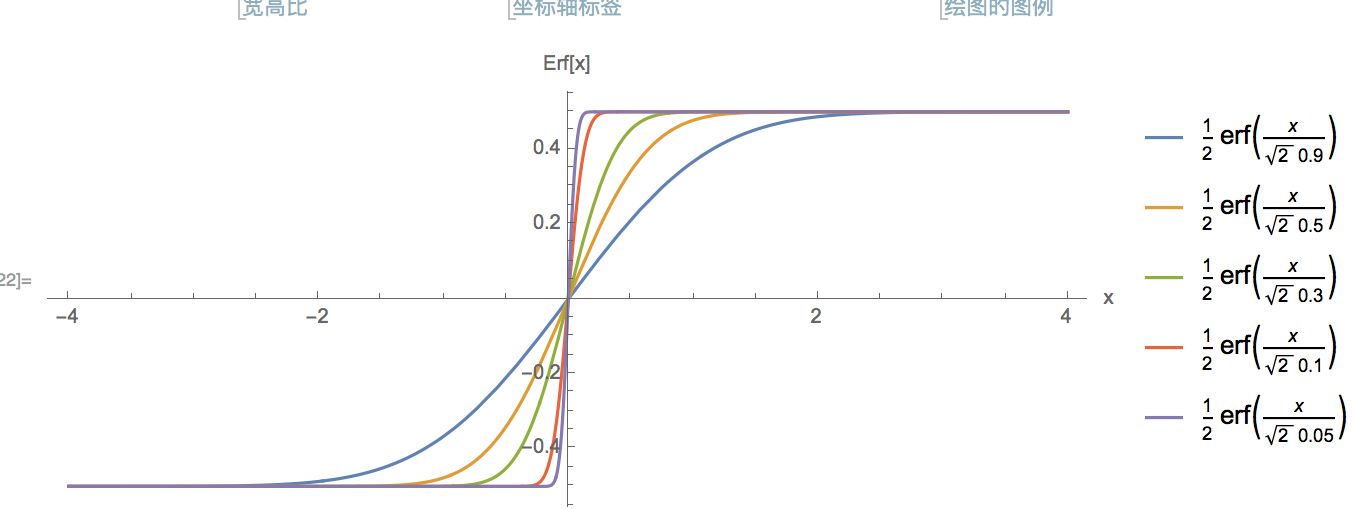
\includegraphics[width=12cm]{./Figures/20180405-gaussian-sigma-value}
  \label{fig:gaussian-kernel-sigma-value}
%
%  \small{Source: PBOC.}
\end{figure}

取$\lim \sigma \rightarrow 0$,内部方差趋近于$0$,此时的误差方程我们成为Heaviside 单位阶跃方程(unit step function)\index{unit step function \dotfill 单位阶跃方程},又称黑维塞方程(Heaviside function)\index{Heaviside function \dotfill 黑维塞方程}。
































\end{subappendices}
